\documentclass{article}
\usepackage{graphicx}
\usepackage{array}
\usepackage{amsmath}
\usepackage{caption}
\usepackage{subcaption}
\usepackage{booktabs}
\usepackage{changepage}
\usepackage{titling}
\usepackage{tikz}
\usepackage{pgfplots}
\usepackage{amsfonts}
\usepackage{multirow}
\usepackage{colortbl} 
\usepackage{bm}
\usepackage{float}
\usepackage[bottom]{footmisc}
\usepackage{arydshln}
\usepackage{wrapfig}
\usepackage{comment}
\usepackage{multicol}
\usepackage{numprint}
\usepackage{appendix}
\usepackage[normalem]{ulem}
\usepackage[a4paper, total={6in,9in}]{geometry}

\usetikzlibrary{calc,patterns,angles,quotes}
\captionsetup[table]{name=\textit{Tabella}}
\renewcommand\maketitlehooka{\null\mbox{}\vfill}
\renewcommand\maketitlehookd{\vfill\null}
\renewcommand*\contentsname{Indice}
\pgfplotsset{compat=1.18}

\title{Esperienza Archimede}
\author{Matteo Herz}
\date{7 Gennaio 2024}

\begin{document}
\begin{titlepage}
	\begin{center}
		\vspace*{4cm}
		
		\textbf{\LARGE Esperienza di laboratorio: Archimede e viscosità}\\
		\vspace{1cm}
		{\LARGE Matteo Herz} \\
		\vspace*{0.2cm}
		{\normalsize  Matricola 1098162}\\
		\vspace{1cm}
        \text{\Large Gruppo 5} \\
        \vspace{1cm}
		{\large 7 Aprile 2024}
		\vspace{2.7cm}
		
		\vfill   %riempie in verticale fino a fine pagina 
		
		\vspace{0.5cm}
		
		{\small Università degli studi di Torino}\\
		{\small Dipartimento di Fisica}\\
		\vspace*{0.1cm}
		
	\end{center}
\end{titlepage}


\newpage
\tableofcontents
\newpage
\section{Scopo dell'esperienza}
Lo scopo dell'esperienza di laboratorio è quello di studiare la spinta di Archimede e, in particolare, come varia in funzione: 
\begin{itemize}
    \item [-] della \textbf{porzione di corpo immerso} nel fluido
    \item [-] della \textbf{densità del fluido} in cui si immerge il corpo
    \item [-] della \textbf{densità del corpo} immerso
\end{itemize}

\noindent Analizzerremo poi in ultima analisi il moto di un oggetto di forma sferica in un liquido, andando a determinare il coefficiente di viscosità di quest'ultimo. 

\begin{comment}
\section{La spinta di Archimede}
Ogni corpo immerso in un fluido subisce l'azione di una forza: 
\begin{itemize}
    \item [-] rivolta \textbf{verso l'alto}
    \item [-] applicata nel \textbf{centro di massa} del sistema
    \item [-] \textbf{pari al peso del volume del fluido spostato}
\end{itemize}
\end{comment}

\vspace{0.5cm}
\section{Strumentazione}
Strumentazione utilizzata: 
\begin{itemize}
    \item [-] Dinamometro \hfill (sensibilità: $0.01\,N$)
    \item [-] Bilancia digitale \hfill (sensibilità: $0.1\,g$)
    \item [-] Picnometro \hfill (No sensibilità)
    \item [-] Calibro a nonio semplice \hfill (sensibilità: $0.05\,mm$)
    \item [-] Calibro elettronico \hfill (sensibilità: $0.01\,mm$)
    \item [-] Righello \hfill (sensibilità: $0.5\,mm$)
    \item [-] Cronometro digitale \hfill (sensibilità: $0.01\,s$)
    \item [-] Becher
    \item [-] 2 fluidi diversi: acqua di rubinetto/acqua di rubinetto + sale
    \item [-] Cilindro graduato 
    \item [-] 5 sfere di materiale diverso (rame, alluminio, ferrro, piombo, ottone)
    \item [-] 14 Sferette di piombo 
\end{itemize}
\vspace{0.5cm}
\section{Spinta di Archimede in funzione di $V_i$}
Per verificare la spinta di Archimede in funzione del volume immerso ($V_i$), abbiamo in primis misurato peso, diametro e altezza del cilindretto utilizzato, con l'usilio di un calibro digitale e di un dinamometro.

Inoltre, per essere più precisi, abbiamo calcolato l'effettiva lunghezza di ognuna delle singole tacche che scandivano l'altezza del cilindro (di base assunte come di $5\,mm$ ognuna tranne per l'ultima, di lunghezza minore), questa volta con un calibro classico.

Di seguito due tabelle riassuntive: 

  \begin{minipage}[c]{0.45\textwidth}
        \centering
            \begin{tabular}{@{}lcc@{}}
        		      \toprule
        		          \textit{Dati} & \textbf{Simbolo} & \textbf{Valore} \\
            		\midrule
            		      \textbf{Diametro} ($mm$) & $d$ & $37.96$\\ [0.1cm]
                            \textbf{Altezza} ($mm$ )& $h$ & $44.30$ \\ [0.1cm]
                            \textbf{Peso} ($N$)& $P_{c}$ & $0.71$\\[0.1cm]
            		\bottomrule
    	   \end{tabular}
        \captionof{table}{\textit{Misurazioni del cilindro}}
    \end{minipage}
    \begin{minipage}[c]{0.45\textwidth}
    	\centering 
            \begin{tabular}{@{}cc@{}}
    		      \toprule
                        \textbf{Tacche Cilindro} & \bm{$h \pm 0.05\,mm$}\\ [0.1cm]
                \midrule
        		        \bm{$1^{a}\;\textit{Tacca}$} & \;$6.30$\\[0.1cm]
                        \bm{$2^{a}\;\text{Tacca}$} & $11.70$\\ [0.1cm]
                        \bm{$3^{a}\;\text{Tacca}$} & $16.15$\\ [0.1cm]
                        \bm{$4^{a}\;\text{Tacca}$} & $21.20$\\ [0.1cm]
                        \bm{$5^{a}\;\text{Tacca}$} & $25.70$\\ [0.1cm]
                        \bm{$6^{a}\;\text{Tacca}$} & $30.60$\\ [0.1cm]
                        \bm{$7^{a}\;\text{Tacca}$} & $35.85$\\ [0.1cm]
                        \bm{$8^{a}\;\text{Tacca}$} & $40.65$\\ [0.1cm]
                        \bm{$9^{a}\;\text{Tacca}$} & $44.30$\\ [0.1cm]
        		\bottomrule
    	\end{tabular}
        \captionof{table}{\textit{Tacche - Altezza cilindro}}
    \end{minipage}
    
\vspace{0.7cm} 
Con l'ausilio del picnometro abbiamo poi calcolato la densità dell'acqua di rubinetto ($\rho_{l}$) con relativo errore. Per fare ciò abbiamo prima pesato con la bilancia il picnometro vuoto ed in seguito pieno, calcolando per differenza la massa d'acqua al suo interno, con il relativo errore dato dalla somma in quadratura delle due incertezze:
\begin{equation*}
    m_{l} = 49.2 \pm 0.14\footnote{Manteniamo due cifre significative per l'errore in quanto arrotondarlo a 0.1 porterebbe a sottostimare l'incertezza di circa il 30\%.}\;g
\end{equation*}
Procediamo a calcolare la densità dell'acqua tenendo conto che il volume del picnometro utilizzato ($49.390\,ml$) non riporta alcuna incertezza per volere del costruttore.

Possiamo dunque utlizzare la formula classica per la propagazione delle incertezze nei i prodotti per determinare l'incertezza da assegnare a $\rho_{l}$: 
\begin{equation}
    \frac{\Delta\rho_{l}}{\rho_{l}} = \frac{\Delta m_{l}}{m_{l}} + \frac{\Delta V_{l}}{V_{l}}
\end{equation}
Assumendo come esatta e dunque priva di incertezza la misura sul volume: 
\begin{equation}
    \frac{\Delta\rho_{l}}{\rho_{l}} = \frac{\Delta m_{l}}{m_{l}} \quad
    \Longrightarrow \quad \Delta\rho_{l} = \frac{\Delta m_{l}}{m_{l}} \rho_{l}
\end{equation}
Ottenendo: 
\begin{equation*}
    \Delta\rho_{l} = 0.996 \pm 0.003\;g/cm^3
\end{equation*}
\\ \indent Andiamo ora a valutare l'entità della spinta di Archiemede immergendo per 10 volte consecutive il cilindro graduato solo fino alla prima tacca, ottenendo una stima della risultante ($P_c - A$).

Valori ottenuti: 
\begin{equation*}
    R = 0.66 \pm 0.002\;N
\end{equation*}

Tenendo conto che la deviazione standard per la media ottenuta è inferiore alla sensibilità del dinamometro utilizzato di $0.01 N$, il risultato corretto risulta essere: 
\begin{equation*}
    R = 0.66 \pm 0.01\;N
\end{equation*}

Sottraendo dunque a $P_c$ il valore ottenuto ($R$) e propagando le incertezze attraverso la somma in quadratura otteniamo una stima per la spinta di Archimede: 
\begin{equation*}
    A = 0.05 \pm 0.014\footnote{Manteniamo due cifre significative per l'errore in quanto arrotondarlo a 0.01 porterebbe a sottostimare l'incertezza di circa il 30\%.}\,N
\end{equation*}
\newpage Ripetiamo ora lo stesso procedimento per le tacche successive del cilindro, limitandoci però a misurare una sola volta la risultante ottenuta e andando a calcolare poi la relativa spinta di Archimede. Il tutto verrà anche poi ripetuto in fase di risalita del cilindro, anche se per il resto dell'esperienza faremo riferimento ai soli valori ottenuti in fase di immersione. 

Ora, per la costruzione del grafico relativo alla spinta di Archimede in funzione del volume immerso $A(V_i)$, andiamo a calcolare il volume del cilindro in corrispondenza delle varie tacche. \\Per propagare l'errore su tali volumi useremo la formula generalare di propagazione degli errori gaussiana, non tenendo conto delle covarianze in quanto le grandezze non sono dipendententi tra loro.
Sostituendo nel nostro caso per il calcolo dell'incertezza relativa al volume di un cilindro: 
\\[0.2cm]
\begin{equation}
    \sigma_V = \sqrt{\left(\pi\,h\,\frac{d}{2} \right)^2 \left(\frac{\sigma_{d}}{2}\right)^2 + \left(\pi \left(\frac{d}{2}\right)^2\right)^2 \left(\sigma_{h}\right)^2}
\end{equation}
\\[0.2cm]
Di seguito una tabella riassuntiva con i volumi immersi ($V_i$), le spinte di Archimede (A) e le relative incertezze. \\ 

\begin{table}[!ht]
\centering
\begin{tabular}{|l|c|c|c|}
\hline
              & \bm{$V_i\;(mm^3)$} & \textbf{Incertezze}\bm{$\;V_i\;(mm^3)$} & \bm{$A\,\pm\,0.014\,N$} \\ \hline
                \bm{$1^a \;\textbf{tacca}$} & 7129.89    & 56.71                     & 0.06                   \\ \hline
                \bm{$2^a \;\textbf{tacca}$} & 13241.22   & 57.01                     & 0.11                   \\ \hline
                \bm{$3^a \;\textbf{tacca}$} & 18277.42   & 57.40                     & 0.17                   \\ \hline
                \bm{$4^a \;\textbf{tacca}$} & 23992.65   & 57.98                     & 0.22                   \\ \hline
                \bm{$5^a \;\textbf{tacca}$} & 29085.42   & 58.62                     & 0.27                   \\ \hline
                \bm{$6^a \;\textbf{tacca}$} & 34630.89   & 59.46                     & 0.32                   \\ \hline
                \bm{$7^a \;\textbf{tacca}$} & 40572.47   & 60.49                     & 0.39                   \\ \hline
                \bm{$8^a \;\textbf{tacca}$} & 46004.77   & 61.56                     & 0.44                   \\ \hline
                \bm{$9^a \;\textbf{tacca}$} & 50135.58   & 62.45                     & 0.48                   \\ \hline
\end{tabular}
\caption{\textit{Volumi e spinte di Archimede a confronto (fluido 1)}}
\end{table}

\subsection{Metodo dei minimi quadrati (fluido 1)}
Ottenuti i nostri dati con le relative incertezze, siamo ora interessati a ricercare quali siano i migliori parametri della relazione funzionale che interrcore tra la spinta di Archimede ed il volume immerso. Siamo cioè interessati a stimare quali siano i migliori parametri $a$ e $b$ della retta teorica $y = a +bx$ che meglio descrive l'andamento dei dati ottenuti sperimentalmene.
Per fare ciò ricorreremo ad un metodo di regressione lineare, ovvero al metodo dei minimi quadrati. Seguirà poi un test del $\chi^2$ per verificare il livello di accordo tra la distribuzione sperimentale dei dati ottenuti e tale retta. \medskip 

Visto che l'errore relativo sulla spinta di Archimede risulta essere in media 26 volte più grande dell'errore relativo legato ai volumi immersi, andremo ad utilizzare come variabile indipendente lungo l'asse delle ascisse il volume e lungo l'asse delle ordinate, con la rispettiva incertezza, la spinta di Archimede. Inoltre, in quanto l'errore relativo su $V_i$ risulta essere trascurabile rispetto all'errore relativo su $A$, non dobbiamo procedere a propagarne l'errore.
\subsubsection{Valori ottenuti}
I valori ottenuti come migliori parametri per la retta dei minimi quadrati ($y=a\,+\,bx$) risultano essere\footnote{Per ricondursi alle u.m. utilizzate nel S.I. si è ricorso ad un semplice conversione delle misure e delle incertezze.}:
\begin{align*}
    a \,&= \,-0.02 \,\pm\, 0.01\;\;N\\
    b \,&= \,\numprint{10041} \,\pm\, 333\;\;\frac{kg}{m^2\cdot s^2}
\end{align*}
\\Inoltre, i valori relativi al coefficiente di correlazione lineare ($r$) e all'errore a posteriori ($\sigma_p$) sono:
\begin{align*}
    r &= 0.998 \\
    \sigma_{p} &= 0.001
\end{align*}
\subsubsection{Grafico - Retta dei minini quadrati}
\begin{figure}[ht]
\centering
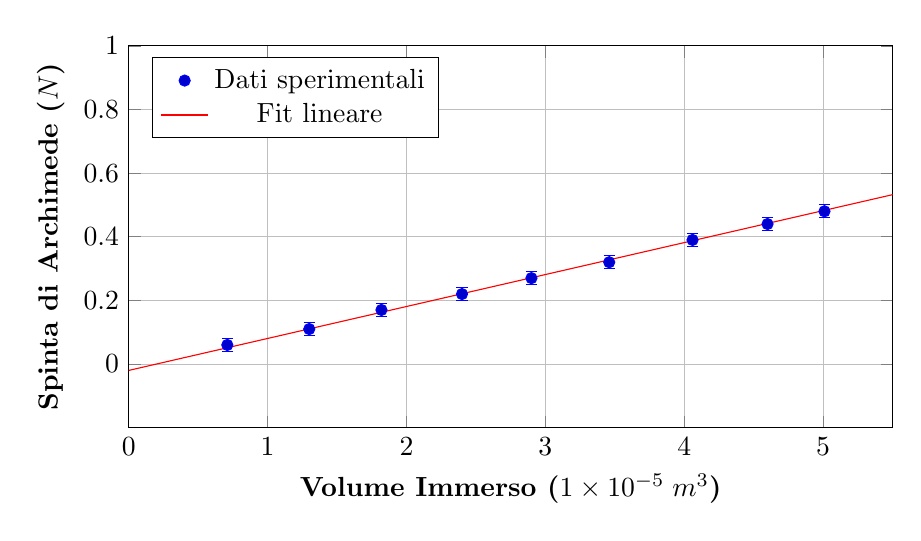
\begin{tikzpicture}
\begin{axis}[
    xlabel={\textbf{Volume Immerso ($1 \times 10^{-5}\;m^3$)}},
    ylabel={\textbf{Spinta di Archimede ($N$)}},
    grid=major,
    xmin=0, xmax=5.5,
    ymin=-0.2, ymax=1,
    xtick={0,1,2,3,4,5},
    ytick={0.0,0.2,0.4,0.6,0.8,1.0},
    width=0.8\textwidth,
    height=0.4\textwidth, % Settaggio delle dimensioni equilibrate
    legend pos=north west,
    scale only axis, % Imposta solo la scala degli assi
]

% Dati del fit lineare con barre di errore
\addplot+[only marks, mark=*, blue, error bars/.cd, y dir=both, y explicit] coordinates {
    (0.71,0.06) +- (0,0.02)
    (1.3,0.11) +- (0,0.02)
    (1.82,0.17) +- (0,0.02)
    (2.4,0.22) +- (0,0.02)
    (2.9,0.27) +- (0,0.02)
    (3.46,0.32) +- (0,0.02)
    (4.06,0.39) +- (0,0.02)
    (4.60,0.44) +- (0,0.02)
    (5.01,0.48) +- (0,0.02)
};

% Fit lineare
\addplot [domain=0:10, red] {0.10041*x + -0.02}; % Modifica i coefficienti in base ai tuoi dati

% Legenda
\legend{Dati sperimentali, Fit lineare}
\end{axis}
\end{tikzpicture}
\label{fig:fit-lineare-con-errore}
\end{figure}

\subsubsection{Test $\chi^2$ - Ipotesi}
\begin{itemize}
    \item[-]\bm{$H_0$}: I dati ottenuti sperimentalmente seguono l'andamento lineare descritto dalla retta dei minimi quadrati.
    \item[-]\bm{$H_1$}: I dati ottenuti sperimentalmente non seguono l'andamento lineare descritto dalla retta dei minimi quadrati.
\end{itemize}

\subsubsection{Test $\chi^2$ - Esito}
\begin{wraptable}{r}{6.5cm}
	\centering
	\begin{tabular}{lc}
		\toprule
		\textbf{Dati} & \textbf{Valori} \\
		\midrule
		Livello di significatività ($\alpha $) & 0.05 \\
		Numero di gradi di libertà & 7\\
		$\chi^2$ critico & 14.07\\
        $\chi^2$ sospetto & 2.167\\
		$\chi^2$ calcolato & 3.45\\
		\bottomrule
	\end{tabular}
	%\captionof{table}{\textit{Test del $\chi^2$ per la verifica della distribuzione dei conteggi}}
\end{wraptable}
Il valore della veriabile $\chi^2$  ottenuto risulta accettabile entro un livello di significatività del 5\%, senza risultare sospetto. Questo conferma l'ipotesi $H_0$, ovvero il corretto andamento lineare della spinta di Archimede in funzione del volume immerso per il nostro set di dati.\medskip

Avendo però ottenuto un termine noto non nullo, in contrasto con l'andamento teorico, siamo tenuti a compiere un test di Gauss per verificarne la compatibilità con il valore teorico $\mu=0\;N$.
\newpage\subsection{Test di Gauss - termine noto}

\subsubsection{Dati del test}
\begin{itemize}
    \item [$\cdot$] Livello di significatività ($\alpha$): 0.05
    \item [-] \textbf{Ipotesi} $H_0$: $a$ è stato estratto da una distribuzione normale avente $\mu = 0\;N$ e deviazione standard pari a $\sigma_{a}$.
    Dunque $a$ e $\mu$ sono tra loro compatibili entro il livello di significatività scelto. 
    \item [-] \textbf{Ipotesi} $H_1$: $a$ non è stato estratto da una distribuzione normale avente $\mu = 0\;N$ e deviazione standard pari a $\sigma_{a}$. Dunque $a$ e $\mu$ non sono tra loro compatibili entro il livello di significatività scelto.
\end{itemize}
\subsubsection{Esito del test}
\begin{equation}
\begin{split}
    Z_{oss} \,&= \,\frac{|\;a - \mu\;|}{\sigma_{a}}
    \\[0.3cm]
    Z_{oss} \,&= \,2 \,> \,1.96 \,= \,Z_{critico} \\[0.2cm]
\end{split}
\end{equation}
Il risultato ottenuto ci porta a rigettare l'ipotesi nulla ($H_0$) e ad accettare l'ipotesi $H_1$. 

Le discrepanze tra il termine noto ottenuto ed il valore teorico $\mu=0\;N$ risultano significative entro il livello di significatività scelto. Nonostante questo, utilizzando un livello di significativà anche solo del 4\%, tale $Z_{oss}$ risulta confrontabile con $\mu=0\;N$ in quanto minore dello $Z_{critico} = 2.6$\,. 
\vspace{0.2cm}

\subsection{Confronto densità (fluido 1)}
Dal coefficiente angolare ottenuto come parametro della retta dei minimi quadrati dal nostro set di dati, è possibile ricavare una stima della densità del fluido. Essendo infatti il coefficiente angolare pari al rapporto tra ascisse e ordinate, nel nostro grafico questo risulta essere pari al rapporto tra la spinta di Archimede e il volume immerso, ovvero: $\rho_{l}\cdot g\,$.

Dunque, dividendo il risultato ottenuto per $g = 9.81\;m\cdot s^{-2}$, otteremo una stima della densità dell'acqua di rubinetto. Numericamente: 
\begin{equation*}
    \rho_l \; = \;\frac{b}{g} \,\pm \,\frac{\sigma_b}{g}\;=\; 1024 \,\pm \,34 \; \frac{kg}{m^3}
\end{equation*}
Il valore ottenuto sperimentalmente a partire dal fit lineare del nostro set di dati è ora confrontabile con il valore ottenuto inizialmente tramite il picnometro. 

Eseguiremo dunque un test di Gauss per vedere se la differenza tra i due ($\bar{\nu} = \rho_{l_{pic}} - \rho_{l_{fit}}$) sia significativa o meno, ovvero se i due valori siano tra loro compatibili. 
\subsubsection{Dati del test}
\begin{itemize}
    \item [$\cdot$] Livello di significatività ($\alpha$): 0.05
    \item [-] \textbf{Ipotesi} $H_0$: $\bar{\nu}\,$ è stato estratto da una distribuzione normale avente $\mu = 0\;\frac{kg}{m^3}$ e deviazione standard pari a $\sigma_{\bar{\nu}}$. Di conseguenza $\rho_{l_{pic}}$ e $\rho_{l_{fit}}$ sono tra loro compatibili entro il livello di significatività scelto.\footnote{L'incertezza $\sigma_{\bar{\nu}}$ è data dalla somma in quadratura di $\sigma_{l_{pic}}$ e $\sigma_{l_{fit}}$}
    \item [-] \textbf{Ipotesi} $H_1$: $\;\bar{\nu}\,$ non è stato estratto da una distribuzione normale avente $\mu = 0\;\frac{kg}{m^3}$ e deviazione standard pari a $\sigma_{\bar{\nu}}$. Di conseguenza $\rho_{l_{pic}}$ e $\rho_{l_{fit}}$ non sono tra loro compatibili entro il livello di significatività scelto.
\end{itemize}
\subsubsection{Esito del test}
\begin{equation*}
\begin{split}
    Z_{oss} \,&= \,0.8 \,< \,1.96 \,= \,Z_{critico} \\[0.2cm]
\end{split}
\end{equation*}
Il risultato ottenuto conferma l'ipotesi nulla ($H_0$): i due valori ottenuti per la densità dell'acqua di rubinetto sono fra loro confrontabili con un livello di significatività del 5\%.
\vspace{0.5cm}
\begin{center}
    \line(1,0){150}
\end{center}
\vspace{0.5cm}
\noindent Ripetiamo ora l'intera procedura sperimentale della sezione precedente variando la densità del fluido, ovvero utilizzando una miscela di acqua di rubinetto e sale. Verrà fatto riferimento a tale miscela come a "fluido 2". Di seguito un riassunto dei valori ottenuti.

\begin{table}[!ht]
\centering
\begin{tabular}{|l|c|c|c|}
\hline
          & \bm{$V_i\;(mm^3)$} & \textbf{Incertezze}\bm{$\;V_i\;(mm^3)$} & \bm{$A\,\pm\,0.014\,N$} \\ \hline
            \bm{$1^a \;\textbf{tacca}$} & 7129.89    & 56.71                     & 0.07                   \\ \hline
            \bm{$2^a \;\textbf{tacca}$} & 13241.22   & 57.01                     & 0.13                   \\ \hline
            \bm{$3^a \;\textbf{tacca}$} & 18277.42   & 57.40                     & 0.19                   \\ \hline
            \bm{$4^a \;\textbf{tacca}$} & 23992.65   & 57.98                     & 0.25                   \\ \hline
            \bm{$5^a \;\textbf{tacca}$} & 29085.42   & 58.62                     & 0.31                   \\ \hline
            \bm{$6^a \;\textbf{tacca}$} & 34630.89   & 59.46                     & 0.37                   \\ \hline
            \bm{$7^a \;\textbf{tacca}$} & 40572.47   & 60.49                     & 0.43                   \\ \hline
            \bm{$8^a \;\textbf{tacca}$} & 46004.77   & 61.56                     & 0.49                   \\ \hline
            \bm{$9^a \;\textbf{tacca}$} & 50135.58   & 62.45                     & 0.53                   \\ \hline
\end{tabular}
\caption{\textit{Volumi e spinte di Archimede a confronto (fluido 2)}}
\end{table}
\subsection{Metodo dei minimi quadrati (fluido 2)}
Ripetiamo quanto riportato in [3.1] con il set di dati riguardante il fluido 2. 
\\Anche in questo caso l'errore relativo sulla spinta di Archimede risulta essere in media 21 volte più grande dell'errore relativo legato ai volumi immersi, il quale si può dunque assumere come trascurabile senza dover propagare l'errore. 

\subsubsection{Valori ottenuti}
I valori ottenuti come migliori parametri per la retta dei minimi quadrati ($y=a\,+\,bx$) risultano essere:
\begin{align*}
    a \,&= \,-0.008 \,\pm\, 0.01\;\;N\\
    b \,&= \,\numprint{10813} \,\pm\, 333\;\;\frac{kg}{m^2\cdot s^2} 
\end{align*}
\\Inoltre, i valori relativi al coefficiente di correlazione lineare ($r$) e all'errore a posteriori ($\sigma_p$) sono:
\begin{align*}
    r &= 0.999 \\
    \sigma_{p} &= 0.003
\end{align*}

\subsubsection{Grafico - Retta dei minini quadrati}
\begin{figure}[H]
\centering
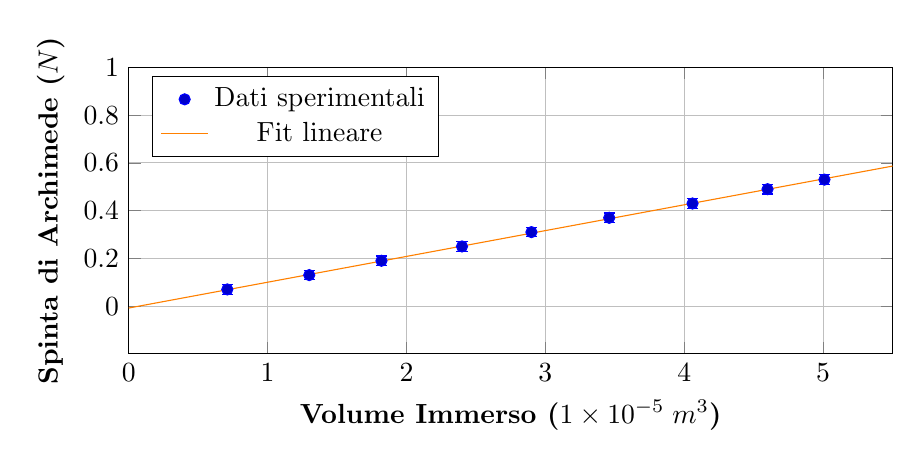
\begin{tikzpicture}
\begin{axis}[
    xlabel={\textbf{Volume Immerso ($1 \times 10^{-5}\;m^3$)}},
    ylabel={\textbf{Spinta di Archimede ($N$)}},
    grid=major,
    xmin=0, xmax=5.5,
    ymin=-0.2, ymax=1,
    xtick={0,1,2,3,4,5},
    ytick={0.0,0.2,0.4,0.6,0.8,1.0},
    width=0.8\textwidth,
    height=0.3\textwidth, % Settaggio delle dimensioni equilibrate
    legend pos=north west,
    scale only axis, % Imposta solo la scala degli assi
]

% Dati del fit lineare con barre di errore
\addplot+[only marks, mark=*, blue, error bars/.cd, y dir=both, y explicit] coordinates {
    (0.71,0.07) +- (0,0.02)
    (1.3,0.13) +- (0,0.02)
    (1.82,0.19) +- (0,0.02)
    (2.4,0.25) +- (0,0.02)
    (2.9,0.31) +- (0,0.02)
    (3.46,0.37) +- (0,0.02)
    (4.06,0.43) +- (0,0.02)
    (4.60,0.49) +- (0,0.02)
    (5.01,0.53) +- (0,0.02)
};

% Fit lineare
\addplot [domain=0:10, orange] {0.10813*x + -0.008}; % Modifica i coefficienti in base ai tuoi dati

% Legenda
\legend{Dati sperimentali, Fit lineare}
\end{axis}
\end{tikzpicture}
\label{fig:fit-lineare-con-errore}
\end{figure}

\subsubsection{Test $\chi^2$ - Ipotesi}
\begin{itemize}
    \item[-]\bm{$H_0$}: I dati ottenuti sperimentalmente seguono l'andamento lineare descritto dalla retta dei minimi quadrati.
    \item[-]\bm{$H_1$}: I dati ottenuti sperimentalmente non seguono l'andamento lineare descritto dalla retta dei minimi quadrati.
\end{itemize}

\subsubsection{Test del $\chi^2$ - Esito}
Il $\chi^2$ ottenuto ad un livello di confidenza del 5\%, risulta "sospetto" in quanto minore di 2.167\,. 
\begin{wraptable}{r}{6.5cm}
	\centering
	\begin{tabular}{@{}lc@{}}
		\toprule
		\textbf{Dati} & \textbf{Valori} \\
		\midrule
		Livello di significatività ($\alpha $) & 0.05 \\
		Numero di gradi di libertà & 7\\
		$\chi^2$ critico & 14.07\\
        $\chi^2$ sospetto & 2.167\\
		$\chi^2$ calcolato & 0.37\\
		\bottomrule
	\end{tabular}
	%\captionof{table}{\textit{Test del $\chi^2$ per la verifica della distribuzione dei conteggi}}
\end{wraptable}
Andando però a consultare l'errore a posteriori ottenuto, pari a 0.003, ci accorgiamo di non star sovrastimando le barre di errore in quanto quest'ultimo risulta essere circa 5 volte più piccolo delle barre di errore utilizzate nell'analisi dati ($0.014\,N$), il cui valore è stato derivato direttamente dalla sensibilità del dinamometro utilizzato ($0.01\,N$), al di sotto del quale non vi è possibilità di andare. Il valore di $r$ suggerisce inoltre una correlazione lineare altamente significativa. 

Preso atto di questo e del fatto che la fase di misurazione della risultante ($R$) avvenisse in condizioni molto stabili, non legate al tempo, possiamo assumere che il $\chi^2$ ottenuto sia effettivamente frutto di un set di punti disposti molto in prossimità della retta dei minimi quadrati, e dunque accettare l'ipotesi nulla ($H_0$).\medskip

In  questo caso non è necessario compiere un test di Gauss per il termine noto in quanto il valore ottenuto ($a = -0.008\;N$) risulta minore della propria incertezza associata ($\sigma_{a} = 0.01\;N$) e dunque compatibile con il valore teorico ($\mu = 0\;N$) entro un livello di significatività del 5\%.

\subsection{Confronto densità (fluido 2)}
Ripetendo il procedeminto esposto in [3.3]:
\begin{equation*}
    \rho_l \; = \;\frac{b}{g} \,\pm \,\frac{\sigma_b}{g}\;=\; 1102 \,\pm \,34 \; \frac{kg}{m^3}
\end{equation*}
Eseguiamo nuovamente un test di Gauss per verificare se la differenza tra la densità calcolata a partire dal coefficiente angolare della retta dei minimi quadrati e quella calcolata attraverso il picnometro ($\bar{\nu} = \rho_{l_{pic}} - \rho_{l_{fit}}$) sia significativa o meno.
\subsubsection{Dati del test}
\begin{itemize}
    \item [$\cdot$] Livello di significatività ($\alpha$): 0.05
    \item [-] \textbf{Ipotesi} $H_0$: $\bar{\nu}\,$ è stato estratto da una distribuzione normale avente $\mu = 0\;\frac{kg}{m^3}$ e deviazione standard pari a $\sigma_{\bar{\nu}}$. Di conseguenza $\rho_{l_{pic}}$ e $\rho_{l_{fit}}$ sono tra loro compatibili entro il livello di significatività scelto\footnote{L'incertezza $\sigma_{\bar{\nu}}$ è data dalla somma in quadratura di $\sigma_{\rho_{l_{pic}}}$ e $\sigma_{\rho_{l_{fit}}}$}.
    \item [-] \textbf{Ipotesi} $H_1$: $\;\bar{\nu}\,$ non è stato estratto da una distribuzione normale avente $\mu = 0\;\frac{kg}{m^3}$ e deviazione standard pari a $\sigma_{\bar{\nu}}$. Di conseguenza $\rho_{l_{pic}}$ e $\rho_{l_{fit}}$ non sono tra loro compatibili entro il livello di significatività scelto.
\end{itemize}
\subsubsection{Esito del test}
\begin{equation*}
\begin{split}
    Z_{oss} \,&= \,0.7 \,< \,1.96 \,= \,Z_{critico} \\[0.2cm]
\end{split}
\end{equation*}
Il risultato ottenuto conferma l'ipotesi nulla ($H_0$): i due valori ottenuti per la densità della miscela di acqua di rubinetto e sale sono fra loro confrontabili ad un livello di significatività del 5\%.


\subsection{Rapporto spinte di Archimede}
\indent Per prevedere il rapporto tra le due spinte di Archimede (a parità di volumi immersi), basta calcolare il rapporto tra le densità dei due fluidi, come si evince facilmente dalla formula stessa.

E' dunque possibile andare a calcolare il rapporto tra le due densità ottenute dai nostri set di dati direttamente dal rapporto dei due coefficienti angolari. 
\\Per verificare l'attendibilità del risultato ottenuto andremo a confrotarlo con il rapporto tra le densità ottenute tramite picnometro, attraverso un test di Gauss. Di seguito i risultati ottenuti: 
\begin{align*}
    \text{Rapporto densità coefficienti angolari ($\theta_c$):}\quad&0.93 \pm 0.04  \\
    \text{Rapporto densità picnometro ($\theta_p$):}\quad&0.92 \pm 0.004
\end{align*}

\noindent Tali incertezze sono state ottenute tramite la formula: 
\begin{equation}
    \sigma_{\theta} = \sqrt{\left(\frac{1}{\rho_2}\right)^2 \left(\sigma_{\rho_1}\right)^2 + \left(-\frac{\rho_1}{(\rho_{2})^2}\right)^2  \left(\sigma_{\rho_2}\right)^2}
\end{equation}


\subsection*{Test di Gauss}
\begin{itemize}
    \item [$\cdot$] Livello di significatività ($\alpha$): 0.05
    \item [-] \textbf{Ipotesi} $H_0$: $\bar{\nu} = |\theta_c - \theta_p|$ è stato estratto da una distribuzione normale avente $\mu = 0$ e deviazione standard pari a $\sigma_{\bar{\nu}}$. Di conseguenza $\theta_c$ e $\theta_p$ sono tra loro compatibili entro il livello di significatività scelto\footnote{L'incertezza $\sigma_{\bar{\nu}}$ è data dalla somma in quadratura di $\sigma_{\theta_c}$ e $\sigma_{\theta_p}$}.
    \item [-] \textbf{Ipotesi} $H_1$: $\bar{\nu} = |\theta_c - \theta_p|$ non è stato estratto da una distribuzione normale avente $\mu = 0$ e deviazione standard pari a $\sigma_{\bar{\nu}}$. Di conseguenza $\theta_c$ e $\theta_p$ non sono tra loro compatibili entro il livello di significatività scelto.
\end{itemize}
\subsubsection*{Esito del test}
\begin{equation*}
\begin{split}
    Z_{oss} \,&= \,0.1 \,< \,1.96 \,= \,Z_{critico} \\[0.2cm]
\end{split}
\end{equation*}
Il rapporto tra le densità ottenute dai coefficienti angolari ($\theta_c$) è compatibile con il rapporto ottenuto tramite le densità ricavate col picnometro ($\theta_p$). 


\section{Spinta di Archimede in funzione di $\rho_c$}
Per verificare l’influenza della densità del corpo immerso ($\rho_c$) per $A$, andiamo a misurare la spinta di Archimede con oggetti che abbiano approsimativamente lo stesso volume, ma di materiale diverso (per quanto dimostrato nel primo punto dell'esperienza, eventuali discrepanze non trascurabili tra i volumi delle 5 sfere dovrebbero essere osservabili nelle differenze tra le varie risultanti).\\
Per fare ciò utilizzeremo 5 sfere rispettivamente di: ottone, rame, alluminio, acciaio e piombo. 
Procediamo dunque a calcolare massa\footnote{Nel calcolo della massa e del peso è inevitabilmente incluso anche il piccolo gancetto di materiale  metallico attaccatto ad ogni sfera, il quale è con molta probabità trascurabile rispetto al resto del corpo, ma di cui non conosciamo la reale entità.}, volume e relativa densità delle sferette. \medskip
\\Diametri, masse e pesi delle sferette: 

\begin{table}[!ht]
\centering
\begin{tabular}{lccccccc}
    \toprule
    \textit{Dati} &\textbf{Ottone} &\textbf{Rame} &\textbf{Alluminio} &\textbf{Acciaio} &\textbf{Piombo} &\textbf{Incertezze } \\
    \midrule
    \textbf{Diametro ($mm$)} &25.24 &25.46 &24.95 &25.32 &25.11 &0.01 \\
    \midrule
    \textbf{Massa ($g$)} &71.5 &77.3 &55.5 &67 &93.3 &0.1 \\
    \midrule
    \textbf{Peso ($N$)} &0.71 &0.77 &0.55 &0.66 &0.92 &0.01 \\
    \bottomrule
\end{tabular}
\end{table}

\noindent Volumi e relative incertezze:
\begin{table}[!ht]
\centering
\begin{tabular}{lcccccc}
    \toprule
    \textit{Dati} &\textbf{Ottone} &\textbf{Rame} &\textbf{Alluminio} &\textbf{Acciaio} &\textbf{Piombo} \\
    \midrule
    \textbf{Volumi ($mm^3$)} &8419.12 &8641.20 &8132.24	&8499.43 &8289.70 \\
    \midrule
    \textbf{Incertezze ($mm^3$)} &10.01	&10.18	&9.78	&10.07	&9.90 \\
    \bottomrule
\end{tabular}
\end{table}

\noindent Le incertezze sui volumi sono state calcolate con la seguente formula: 
\begin{equation}
    \sigma_V = \sqrt{\left(\frac{\pi d^2}{2}\right)^2 \left(\sigma_{d}\right)^2}
\end{equation}
Dove:
\vspace{0.2cm}
\begin{itemize}
    \item [-] $d$ è il diametro della sfera
    \item [-] $\sigma_{d}$ è l'errore associato al diametro $d$
\end{itemize}
\medskip
\noindent Di seguito le densità\footnote{Le incertezze relative alla densità della sfera di alluminio e alla sfera in piombo vengono riportate come tali in quanto approssimarle a 0.01 porterebbe nel primo caso a sovrastimare l'errore del 20\% e nel secondo caso ad una sottostima di circa il 30\%.} ottenute:
\begin{table}[!ht]
\centering
\begin{tabular}{lcccccc}
    \toprule
    \textit{Dati} &\textbf{Ottone} &\textbf{Rame} &\textbf{Alluminio} &\textbf{Acciaio} &\textbf{Piombo} \\
    \midrule
    \textbf{Densità ($g\cdot cm^{-3}$)} &8.49 &8.95 &6.82 &7.88 &11.25 \\
    \midrule
    \textbf{Incertezze ($g\cdot cm^{-3}$)} &0.01	&0.01	&0.008	&0.01	&0.014 \\
    \bottomrule
\end{tabular}
\end{table}

\noindent Le incertezze sulle densità sono state calcolate con la seguente formula:
\begin{equation}
    \sigma_{\rho} = \sqrt{\left(\frac{1}{V}\right)^2 \left(\sigma_{m}\right)^2 + \left(-\frac{m}{V^2}\right)^2  \left(\sigma_{V}\right)^2}
\end{equation}
\newpage dove:
\begin{itemize}
    \item [-] $\sigma_{m}$ è l'errore associato alla massa $m$
    \item [-] $\sigma_{V}$ è l'errore associato al volume $V$
\end{itemize}
\vspace{0.3cm} 
Calcoliamo poi la risultante ($P_c - A$) immergendo le sfere (sia nel fluido 1 che nel fluido 2), e in seguito, per differenza, la relativa spinta di Archimede.

\begin{table}[H]
\centering
\renewcommand{\arraystretch}{1.3}
\begin{tabular}{lccccccc}
    \multicolumn{7}{c}{\textbf{FLUIDO 1}} \\
    \toprule
    \textit{Dati} &\textbf{Ottone} &\textbf{Rame} &\textbf{Alluminio} &\textbf{Acciaio} &\textbf{Piombo} &\textbf{Incertezze} \\
    \midrule
    \textbf{Risultante ($N$)} &0.63 &0.68	&0.47 &0.58	&0.84 &0.1\\
    \midrule
    \textbf{Archimede ($N$)} &0.8 &0.9 &0.8 &0.8 &0.8 &0.014\\ 
    \bottomrule
\end{tabular}
\end{table}

\begin{table}[H]
\centering
\renewcommand{\arraystretch}{1.3}
\begin{tabular}{lccccccc}
    \multicolumn{7}{c}{\textbf{FLUIDO 2}} \\
    \toprule
    \textit{Dati} &\textbf{Ottone} &\textbf{Rame} &\textbf{Alluminio} &\textbf{Acciaio} &\textbf{Piombo} &\textbf{Incertezze} \\
    \midrule
    \textbf{Risultante ($N$)} &0.62 &0.68	&0.47 &0.57	&0.83 &0.1 \\
    \midrule
    \textbf{Archimede ($N$)} &0.9 &0.9 &0.8 &0.9 &0.9 &0.014\\ 
    \bottomrule
\end{tabular}
\end{table}
\vspace{0.3cm}

Le spinte di Archimede ottenute risultano tutte uguali tra loro, per entrambi i fluidi, a meno della spinta registrata per la sfera di rame (fluido 1) e per la sfera di alluminio (fluido 2), che risultano infatti essere rispettivamente la sfera con volume maggiore e la sfera con volume minore; ciò è perfettamente in accordo con quanto dimostrato nel primo punto dell'esperienza. 

Nonostante questo, la discrepanza con le altre spinte di Archimede risulta essere contenuta entro una volta l'incertezza associata a quest'ultima, pari a $0.014\;N$, di conseguenza non è necessario effettuare un test di Gauss, ma possiamo direttamente affermare che esse sono confrontabili tra loro con un livello di significatività del 5\%. \medskip

Oltre a confermare quanto osservato nel primo punto dell'esperinza, dai risultati ottenuti possiamo anche apprezzare la dipendenza della spinta di Archimede dalla densità del fluido, osservando come mediamente la spinta di Archimede registrata per il fluido 2 (miscela di acqua di rubinetto $+$ sale, dunque più densa della sola acqua di rubinetto) risulti maggiore di quella registrata per il fluido 1.\medskip

In ultima analisi possiamo dunque dedurre come la spinta di Archimede non dipenda dalla densità dei corpi immersi, in quanto le discrepanze osservate tra sfere aventi densità differenti non sono tra loro significative.

\section{Viscosità e spinta di Archimede}
La scopo di quest'ultima parte dell'esperienza di laboratorio sarà quella di studiare il moto di un oggetto di forma sferica in un liquido e determinare il coefficiente di viscosità di quest'ultimo.

Per fare ciò utilizzeremo 14 sferette di piombo, le quali verranno fatte cadere una alla volta in un cilindro graduato riempito di shampoo. Verranno presi i tempi di caduta con un cronometro digitale e poi calcolate le rispettive velocità medie da cui proveremo a stimare il coefficiente di viscosità $\eta$. Tale coefficiente verrà calcolato in due modi: prima non tenendo conto della spinta di Archimede ed in seguito tenendo conto della spinta di Archimede, per procedere poi ad un confronto finale tra i due valori ottenuti.\medskip

Per prima cosa pesiamo le palline tutte insieme con un bilancia e ne stimiamo la massa media ed il relativo errore\footnote{Valori ottenuti dividendo la massa totale e la relativa incertezza (sensibilità strumento) per 14}. Ne calcoliamo poi i 14 diametri con un calibro elettronico e ne stimiamo il diametro medio e l'incertezza\footnote{L'incertezza associata è la deviazione standard della media dei 14 diametri}. Una volta ottenuto il diametro, calcoliamo il volume medio, l'incertezza associata [\,formula (6)\,] e per finire la densità media con la relativa incertezza [\,formula (7)\,].
Di seguito una tabella riassuntiva: 

\begin{table}[H]
    \centering
    \renewcommand{\arraystretch}{1.2} % aumenta lo spazio tra le righe
    \begin{tabular}{|l|c|c|c|}
        \hline
        \textit{Dati} & \textbf{Valori Ottenuti} & \textbf{Incertezze} & \textbf{u.m.}  \\
        \hline
        \textbf{Peso totale} & 62.4 & 0.1 & $g$ \\
        \hline
        \textbf{Peso medio} & 4.46 & 0.007 & $g$\\
        \hline
        \textbf{Diametro medio} & 10.26 & 0.01 & $mm$\\
        \hline
        \textbf{Volume medio} & 564.92 & 1.16 & $mm^3$\\
        \hline
        \textbf{Densità media} & 7.89 & 0.02 & $g\cdot cm^{-3}$\\
        \hline
    \end{tabular}
    \caption{\textit{Risultati delle misurazioni per le 14 sferette}}
\end{table}

\vspace{0.2cm}
Suddividendo poi il becher in 3 segmenti di altezza $h = 67 \pm 0.5\,mm$, andiamo a far cadere le palline prendendone i tempi di passaggio alla fine del primo, del secondo e del terzo intevallo. Calcoliamo poi per ogni segmento il tempo di percorrenza medio, la velocità media ed i relativi errori. La tabella con tutti i tempi registrati è consultabile in appendice. Di seguito una tabella riassuntiva dei valori ottenuti:

\begin{table}[!ht]
\centering
\renewcommand{\arraystretch}{1.2} % aumenta lo spazio tra le righe
\begin{tabular}{|c|c|c|c|}
\hline
\textbf{Segmento} & \textbf{Tempo Medio ($s$)} & \textbf{Tempo di percorrenza medio ($s$)} & \textbf{Velocità media ($mm\cdot\,s^{-1}$)} \\
\hline
\textbf{1°} & $1.05 \pm 0.02 $ & $1.05 \pm 0.02$ & $64.1 \pm 1.5$ \\
\textbf{2°} & $2.06 \pm 0.04 $ & $1.01 \pm 0.05$ & $66.3 \pm 3.1$ \\
\textbf{3°} & $3.00 \pm 0.04 $ & $0.94 \pm 0.05$ & $71.6 \pm 4.1$ \\
\hline
\end{tabular}
\caption{\textit{Tempi e velocità medie per le 14 sferette}}
\end{table}

Le incertezze corrispondenti alle medie dei tempi di passaggio (indicate nella tabella con "Tempo Medio") alla fine del primo, secondo e terzo segmento, sono state ottenute come le deviazioni standard delle medie delle 14 misure effettuate per ognuno dei 3 segmenti. \\L'incertezza associata al tempo di percorrenza medio ($t_m$) è data dalla semplice somma in quadratura, mentre l'incertezza relativa alla velocità media ($v_m$) è stata ottenuta dalla seguente formula: 
\vspace{0.1cm}
\begin{equation}
    \sigma_{v_m} = \sqrt{\left(\frac{1}{t_m}\right)^2\left(\sigma_{h}\right)^2 + \left(-\frac{h}{t_{m}^2}\right)^2 \left(\sigma_{t_m}\right)^2}
\end{equation}
\vspace{0.3cm}

Andiamo ora a compiere 3 test di Gauss per verificare se le velocità medie nei rispettivi segmenti sono tra loro compatibili o meno.
\subsection{Test di Gauss ($v_1 - v_2$)}
\begin{itemize}
    \item [$\cdot$] Livello di significatività ($\alpha$): 0.05
    \item [-] \textbf{Ipotesi} $H_0$: $\bar{\nu} = |v_1 - v_2|$ è stato estratto da una distribuzione normale avente $\mu = 0\;m\cdot s^{-1}$ e deviazione standard pari a $\sigma_{\bar{\nu}}$. Di conseguenza $v_1$ e $v_2$ sono tra loro compatibili entro il livello di significatività scelto\footnote{L'incertezza $\sigma_{\bar{\nu}}$ è data dalla somma in quadratura di $\sigma_{v_1}$ e $\sigma_{v_2}$}.
    \item [-] \textbf{Ipotesi} $H_1$: $\bar{\nu} = |v_1 - v_2|$ non è stato estratto da una distribuzione normale avente $\mu = 0\;m\cdot s^{-1}$ e deviazione standard pari a $\sigma_{\bar{\nu}}$. Di conseguenza $v_1$ e $v_2$ non sono tra loro compatibili entro il livello di significatività scelto.
\end{itemize}
\subsubsection{Esito del test}
\begin{equation*}
\begin{split}
    Z_{oss} \,&= \,0.8 \,< \,1.96 \,= \,Z_{critico} \\[0.2cm]
\end{split}
\end{equation*}
Il risultato ottenuto conferma l'ipotesi nulla ($H_0$): la velocità media nel primo segmento ($v_1$) è compatibile con la velocità media nel secondo segmento ($v_2$) ad un livello di significatività del 5\%.
\vspace{0.3cm}

\subsection{Test di Gauss ($v_1 - v_3$)}
\begin{itemize}
    \item [$\cdot$] Livello di significatività ($\alpha$): 0.05
    \item [-] \textbf{Ipotesi} $H_0$: $\bar{\nu} = |v_1 - v_3|$ è stato estratto da una distribuzione normale avente $\mu = 0\;m\cdot s^{-1}$ e deviazione standard pari a $\sigma_{\bar{\nu}}$. Di conseguenza $v_1$ e $v_3$ sono tra loro compatibili entro il livello di significatività scelto\footnote{L'incertezza $\sigma_{\bar{\nu}}$ è data dalla somma in quadratura di $\sigma_{v_1}$ e $\sigma_{v_3}$}.
    \item [-] \textbf{Ipotesi} $H_1$: $\bar{\nu} = |v_1 - v_3|$ non è stato estratto da una distribuzione normale avente $\mu = 0\;m\cdot s^{-1}$ e deviazione standard pari a $\sigma_{\bar{\nu}}$. Di conseguenza $v_1$ e $v_3$ non sono tra loro compatibili entro il livello di significatività scelto.
\end{itemize}
\subsubsection{Esito del test}
\begin{equation*}
\begin{split}
    Z_{oss} \,&= \,1.7 \,< \,1.96 \,= \,Z_{critico} \\[0.2cm]
\end{split}
\end{equation*}
Il risultato ottenuto conferma l'ipotesi nulla ($H_0$): la velocità media nel primo segmento ($v_1$) è compatibile con la velocità media nel terzo segmento ($v_3$) ad un livello di significatività del 5\%.
\vspace{0.3cm}

\subsection{Test di Gauss ($v_2 - v_3$)}
\begin{itemize}
    \item [$\cdot$] Livello di significatività ($\alpha$): 0.05
    \item [-] \textbf{Ipotesi} $H_0$: $\bar{\nu} = |v_2 - v_3|$ è stato estratto da una distribuzione normale avente $\mu = 0\;m\cdot s^{-1}$ e deviazione standard pari a $\sigma_{\bar{\nu}}$. Di conseguenza $v_2$ e $v_3$ sono tra loro compatibili entro il livello di significatività scelto\footnote{L'incertezza $\sigma_{\bar{\nu}}$ è data dalla somma in quadratura di $\sigma_{v_2}$ e $\sigma_{v_3}$}.
    \item [-] \textbf{Ipotesi} $H_1$: $\bar{\nu} = |v_2 - v_3|$ non è stato estratto da una distribuzione normale avente $\mu = 0\;m\cdot s^{-1}$ e deviazione standard pari a $\sigma_{\bar{\nu}}$. Di conseguenza $v_2$ e $v_3$ non sono tra loro compatibili entro il livello di significatività scelto.
\end{itemize}
\subsubsection{Esito del test}
\begin{equation*}
\begin{split}
    Z_{oss} \,&= \,1.0 \,< \,1.96 \,= \,Z_{critico} \\[0.2cm]
\end{split}
\end{equation*}
Il risultato ottenuto conferma l'ipotesi nulla ($H_0$): la velocità media nel secondo segmento ($v_2$) è compatibile con la velocità media nel terzo segmento ($v_3$) ad un livello di significatività del 5\%.
\subsubsection{Conclusioni - confronto velocità}
Al contrario di quanto ci aspetteremmo, la velocità media sui 3 segmenti non risulta diminuire durante la fase di caduta, bensì aumentare, da quanto si evince nella \textit{Tabella 6}. A primo impatto questo sembrerebbe contradditorio, in quanto le sferette, essendo soggette alla forza di attrito viscoso, dovrebbero raggiungere la velocità limite già nel primo tratto del cilindro graduato.

Nonostante questo però, applicando un test di Gauss le 3 velocità risultano tutte tra loro compatibili viste le incertezze. Le differenze osservate, così come il fatto che la velocità sembri aumentare, potrebbero quindi essere frutto di fluttuazioni statistiche, e della prontezza/riflessi in fase di presa dati, contando che la pallina andava seguita ad occhio mentre cadeva lungo il cilindro graduato, con possibili errori di parallasse.

Di conseguenza, al fronte di tali incertezze, le differenze riscontrate tra le 3 velocità risultano di fatto trascurabili, indicando come nonostante i valori crescenti ottenuti per quest'ultime, le sferette possano in realtà aver raggiunto mediamente la velocità limite già nel primo tratto del cilindro graduato. 

\subsection{Coefficiente di viscosità: $\eta$}
Andiamo ora a calcolare il coefficiente di viscosità $\eta$ in due modi diversi: prima non tenendo conto della spinta di Archimede e poi in secondo luogo tenendo conto di quest'ultima. 

Se la spinta di Archimede non dovesse essere trascurabile, come ci aspettiamo, le discrepanze tra le due stime di $\eta$ dovrebbero risultare significative entro un livello di significatività del 5\%.
\vspace{0.2cm}
\subsubsection{\bm{$\eta$} trascurando Archimede}
Calcoliamo la velocità media, coincidente con la velocità limite ($v_l$), sull'intero percorso, ovvero sullo spazio totale coperto dai 3 segmenti di altezza $h = 67 \pm 0.5\,mm$, tramite il tempo medio di passaggio alla fine del terzo segmento ($t_m$), pari $3.00 \pm 0.04\,s$.
\vspace{0.2cm}

\begin{equation}
        v_{l} = \;\frac{S_{tot}}{t_m}\; = \;\frac{3\cdot h}{t_m} \\[0.3cm]
\end{equation}
\begin{equation}
    \sigma_{v_l} = \sqrt{\left(\frac{1}{t_m}\right)^2\left(\sigma_{S_{tot}}\right)^2 + \left(\frac{-S_{tot}}{t_{m}^2}\right)^2 \left(\sigma_{t_m}\right)^2}
\end{equation}
\\[0.2cm]
\noindent Numericamente: 
\begin{equation*}
        v_{l} = \;67.05 \;\pm \;0.94\;\frac{mm}{s}
\end{equation*}
\\
Ora possiamo calcolare il coefficiente di viscosità $\eta$ con la relativa incertezza: 
\vspace{0.2cm}
\begin{equation}
    \eta = \frac{m\,g}{6\,\pi\,\frac{d}{2}\,v_l}
\end{equation}
\begin{equation}
     \sigma_{\eta} = \sqrt{\left(\frac{g}{6\pi \frac{d}{2} v_{l}}\right)^2 \left(\sigma_{m}\right)^2 + \left(-\frac{mg}{6\pi \left(\frac{d}{2}\right)^2 v_{l}}\right)^2 \left(\frac{\sigma_{d}}{2}\right)^2 + \left(-\frac{mg}{6\pi \frac{d}{2} v_{l}^2}\right)^2 \left(\sigma_{v_{l}}\right)^2} \\[0.4cm]
\end{equation}
\vspace{0.2cm}
\noindent Numericamente: 
\begin{equation*}
    \eta = \;6.75\; \pm\; 0.09 \,\frac{kg}{m\cdot s}
\end{equation*}
\vspace{0.3cm}

\subsubsection{\bm{$\eta$} includendo Archimede}
Ricalcoliamo $\eta$ e la relativa incertezza utilizzando la formula completa, tenente conto della spinta di Archimede, e utilizzando la densità dello shampoo ($\rho_l = 1.04\,\pm\,0.04\,g\cdot cm^{-3}$) nota sperimentalmente:
\vspace{0.2cm}
\begin{equation}
    \eta = \frac{(\rho_c - \rho_l)\,Vg}{6\,\pi\,\frac{d}{2}\,v_l}
\end{equation}

\centerline{
  \begin{minipage}{\linewidth}
    \begin{align*}
      \sigma_{\eta} = \sqrt{\left(\frac{Vg}{6\pi \frac{d}{2} v_{l}} \sigma_{\rho_c}\right)^2 + \left(-\frac{Vg}{6\pi \frac{d}{2} v_{l}} \sigma_{\rho_l}\right)^2 + \left(\frac{(\rho_c - \rho_l)g}{6\pi \frac{d}{2} v_{l}} \sigma_{V}\right)^2 + \left(-\frac{(\rho_c - \rho_l)Vg}{6\pi \left(\frac{d}{2}\right)^2 v_{l}}\, \frac{\sigma_{d}}{2}\right)^2 + \left(-\frac{(\rho_c - \rho_l)Vg}{6\pi \frac{d}{2} v_{l}^2} \sigma_{v_{l}}\right)^2}
    \end{align*}
  \end{minipage}
}
\vspace{0.9cm}
\noindent Numericamente: 
\begin{equation*}
    \eta = \;5.86\; \pm\; 0.09 \,\frac{kg}{m\cdot s}
\end{equation*}

\subsection{Test di Gauss - $\eta$}
Eseguiamo infine un ultimo test di Gauss per verificare la compatibilità tra i due coefficienti di viscosità appena calcolati. Indicheremo con $\eta_1$ il coefficiente calcolato senza tener conto della spinta di Archimede e con $\eta_2$ quello tenente conto della spinta di Archimede.

\begin{itemize}
    \item [$\cdot$] Livello di significatività ($\alpha$): 0.05
    \item [-] \textbf{Ipotesi} $H_0$: $\bar{\nu} = |\eta_1 - \eta_2|$ è stato estratto da una distribuzione normale avente $\mu = 0\;\frac{kg}{m\cdot s}$ e deviazione standard pari a $\sigma_{\bar{\nu}}$. Di conseguenza $\eta_1$ e $\eta_2$ sono tra loro compatibili entro il livello di significatività scelto\footnote{L'incertezza $\sigma_{\bar{\eta}}$ è data dalla somma in quadratura di $\sigma_{\eta_1}$ e $\sigma_{\eta_2}$}.
    \item [-] \textbf{Ipotesi} $H_1$: $\bar{\nu} = |\eta_1 - \eta_2|$ non è stato estratto da una distribuzione normale avente $\mu = 0\;\frac{kg}{m\cdot s}$ e deviazione standard pari a $\sigma_{\bar{\nu}}$. Di conseguenza $\eta_1$ e $\eta_2$ non sono tra loro compatibili entro il livello di significatività scelto.
\end{itemize}
\subsubsection{Esito del test}
\begin{equation*}
\begin{split}
    Z_{oss} \,&= \,6.8 \,> \,1.96 \,= \,Z_{critico} \\[0.3cm]
\end{split}
\end{equation*}
Il risultato ottenuto ci porta a rigettare l'ipotesi nulla ($H_0$) e ad accettare l'ipotesi $H_1$. 
\\La discrepanza ottenuta tra $\eta_1$ e $\eta_2$ risulta significativa, indicando come la spinta di Archimede non sia trascurabile. Ne deduciamo dunque che il valore precedentemente calcolato per $\eta_1$ è affetto da errore sistematico.

\newpage \section{Conclusioni}
\begin{itemize}
    \item [\textbf{1)}]\textbf{Spinta di archimede in funzione di \bm{$V_i$}.} 
    \\Grazie all'ausilio della rigressione lineare (metodo dei minimi quadrati) e del test del $\chi^2$, abbiamo verificato positivamente per entrambi i fluidi l'andamento lineare della spinta di Archimede in funzione del volume immerso. Inoltre, le densità ottenute a partire dei coefficienti angolari delle rette, sono risultate compatibili, ad un livello di significatività del 5\%, con le densità ottenute sperimentalmente tramite il picnometro.
    \\Questi risultati evidenziano un'accurata e precisa acquisizione dei dati, come mostrato anche dal valore sospetto del $\chi^2$ ottenuto per il fluido 2.
    
    \item [\textbf{2)}] \textbf{Spinta di archimede in funzione di \bm{$\rho_c$}.} 
    \\I risultati ottenuti confrontando le spinte di Archimede per sfere di densità differenti mostrano come quest'ultima non dipenda in nessun modo dalla densità del corpo immerso, bensì dal volume del corpo immerso e dalla densità del liquido. 
    \\Non è stato necessario effettuare un test di Gauss per verificare tale risultato in quanto nel peggiore dei casi la discrepanza tra le diverse spinte di Archimede è risultata essere contenuta entro una volta l'incertezza associata a tali spinte. Di conseguenza le spinte di Archimede ottenute sono risultate tutte tra loro confrontabili con un livello di significatività del 5\%.

    \item [\textbf{3)}] \textbf{Viscosità} 
    \\Le 3 velocità medie ottenute per le sferette nei relativi segmenti sono risultate tutte tra loro confrontabili con un livello di significativià del 5\%. Nonostante i valori ottenuti possano in primo luogo mostrare un'apparente accellerazione delle sferette lungo tutto il percorso, le "ampie" incertezze associate e l'effetto delle fluttuazioni statistiche rendono tra loro le velocità compatibili, mostrando come mediamente le sferette possano in realtà aver raggiunto la velocità limite prima della fine del 1° segmento.
    \\Infine, per quanto riguarda il coefficiente di viscosità, i due valori di $\eta$ calcolati non sono risultati tra loro confrontabili ad un livello di significativà del 5\%, mostrando un'errore sistematico nel calcolo di $\eta_1$ e dunque come la spinta di Archimede non sia una forza trascurabile per le sferette immerse nello shampoo.
    
\end{itemize}

\newpage
\appendix % Inizia l'appendice
\section*{Appendice A} % Titolo dell'appendice senza numerazione
\addcontentsline{toc}{section}{Appendice A} % Aggiungi il titolo all'indice senza numerazione
Dati registrati con il cronometro digitale per i tempi di passaggio alla fine dei vari segmenti del cilindro graduato.

\begin{table}[htbp]
    \centering
    \captionof{table}{\textit{Tempi registrati in laboratorio}}
    \begin{minipage}{0.45\textwidth}
    \centering
    \begin{tabular}{lcc}
        \toprule
        \textbf{Lap }& \textbf{Segmento} & \textbf{Tempi ($s$)} \\
        \midrule
        1 & 1° segmento & 1.18 \\
          & 2° segmento & 2.19 \\
          & 3° segmento & 3.20 \\
        \midrule
        2 & 1° segmento & 1.15 \\
          & 2° segmento & 2.16 \\
          & 3° segmento & 3.21 \\
        \midrule
        3 & 1° segmento & 1.05 \\
          & 2° segmento & 2.06 \\
          & 3° segmento & 2.94 \\
        \midrule
        4 & 1° segmento & 1.15 \\
          & 2° segmento & 2.16 \\
          & 3° segmento & 3.09 \\
        \midrule
        5 & 1° segmento & 1.13 \\
          & 2° segmento & 2.39 \\
          & 3° segmento & 3.07 \\
        \midrule
        6 & 1° segmento & 1.03 \\
          & 2° segmento & 2.12 \\
          & 3° segmento & 2.96 \\
        \midrule
        7 & 1° segmento & 1.11 \\
          & 2° segmento & 2.12 \\
          & 3° segmento & 3.09 \\
        \bottomrule
    \end{tabular}
    \end{minipage}\hfill
    \begin{minipage}{0.45\textwidth}
    \centering
    \begin{tabular}{lcc}
        \toprule
        \textbf{Lap} & \textbf{Segmento} & \textbf{Tempi ($s$)} \\
        \midrule
        8 & 1° segmento & 1.03 \\
          & 2° segmento & 1.91 \\
          & 3° segmento & 3.09 \\
        \midrule
        9 & 1° segmento & 0.97 \\
          & 2° segmento & 1.90 \\
          & 3° segmento & 2.83 \\
        \midrule
        10 & 1° segmento & 0.96 \\
           & 2° segmento & 2.09 \\
           & 3° segmento & 2.93 \\
        \midrule
        11 & 1° segmento & 1.06 \\
           & 2° segmento & 2.11 \\
           & 3° segmento & 3.00 \\
        \midrule
        12 & 1° segmento & 0.99 \\
           & 2° segmento & 1.92 \\
           & 3° segmento & 2.85 \\
        \midrule
        13 & 1° segmento & 0.91 \\
           & 2° segmento & 1.96 \\
           & 3° segmento & 2.93 \\
        \midrule
        14 & 1° segmento & 0.92 \\
           & 2° segmento & 1.81 \\
           & 3° segmento & 2.78 \\
        \bottomrule
    \end{tabular}
    \end{minipage}
\end{table}



\end{document}